%%%%%%%%%%%%%%%%%%%%%%%%%%%%%%%%%%%%%%%%%%%%%%%%%%%%%%%%%%
%%                                                      %% 
%%      Crowdmark LaTeX Exam Template v0.1              %%
%%                2013-09-20                            %%
%%                                                      %%
%%           Comments or Suggestions?                   %%
%%          email: info@crowdmark.com                   %% 
%%%%%%%%%%%%%%%%%%%%%%%%%%%%%%%%%%%%%%%%%%%%%%%%%%%%%%%%%%

\documentclass[14pt, oneside]{memoir}
\pagestyle{plain}

\usepackage{array, amssymb}
\extrarowheight=5pt{\tiny }
\voffset=-20pt
\textheight=9.5in
%\topmargin=2in
\usepackage{mathtools}
%\usepackage{amsthm}
\usepackage{xcolor}
\usepackage{enumitem}
\newcommand{\erf}{\operatorname{erf}}


\parindent=0pt
\begin{document}


{\textbf{ECO 209 Test 1}}
\vskip 10pt

2024-11-13
\vskip 30pt

\begin{tabular}[t]{l}
%\hline
\hphantom{Last name Last nameLast nameLast name}\\[-15pt]
Last name:  \dotfill  \\
\vspace{0.2cm}

First name: \dotfill  \\

\vspace{0.2cm}
Student ID: \dotfill
%\hline
 \end{tabular}

	\begin{center}
	\fbox{\fbox{\parbox{5.5in}{\centering
				Instructions:
				\begin{enumerate}
					\item Explain all of your answers. Show all necessary steps. Be concise.
					\item Read each question carefully before attempting to answer.
					\item Write legibly and preferably in pen.
					
					\item Make all extra assumptions that you consider necessary but make sure to state them clearly.
					\item Make sure to label all your diagrams appropriately.
					%\item You have to hand in the exam sheet. % and any booklets (if any). Please insert additional booklets inside the first booklet before you hand them in.
					%\item If you are using extra booklets, make sure to write your name on each of your books and indicate the order of the booklets (e.g., label them 1 of 2, and 2 of 2).
					\item DO NOT turn this page until instructed.
				\end{enumerate}
				
				
				
				
				Time: 100 minutes
				
				Total Score: 20+10+10+15+15+30=100 points; Pages: 20
				
				ONLY Non-Programmable Calculators is ALLOWED
	}}}
\end{center}

\quad
\newpage


\begin{enumerate}[label=\textbf{\arabic*.}, itemsep=15pt]

\item \textbf{(20  pts)}\label{P1} Consider an economy with two consumption goods (\(C_1\) and \(C_2\)) and two investment goods (\(I_1\) and \(I_2\)). The table below shows the price (\(P\)) and quantity (\(Q\)) of the consumption and investment goods (e.g., $P_{C1}$ is the price of consumption good 1). Use the table to answer the questions below. \textit{Show all the formulas used in the calculations}.

\begin{table}[htbp]
	\centering
	
	\begin{tabular}{rrrrrrrrr}
		& $P_{C1}$ & $Q_{C1}$ & $P_{C2}$ & $Q_{C2}$ & $P_{I1}$ & $Q_{I1}$ & $P_{I2}$ & $Q_{I2}$ \\ \hline
		2020  & 90     & 80    & 12    & 40    & 20    & 10    & 110   & 14 \\
		2021  & 95     & 160   & 14    & 45    & 22    & 11    & 112   & 15 \\
		2022  & 100    & 280   & 30    & 45    & 24    & 14    & 115   & 16 \\ \hline
	\end{tabular}%
\end{table}%

\begin{enumerate}[label=(\alph*)]
	\item \textbf{(3  pts)}  The table below presents real consumption, real investment, and real GDP, using the prices from 2020, 2021, and 2022. Please complete parts (i) to (ix).
	
	\begin{table}[htbp]
		\centering
		\begin{tabular}{lccc}
			Base year = 2020 & C     & I     & Y \\ \hline
			2020  & i)  & 1740  & -- \\
			2021  & 14940 & ii)  & 16810 \\
			2022  & 25740 & 2040  & iii) \\ \hline
			&       &       &  \\
			Base year = 2021 & C     & I     & Y \\ \hline
			2020  & iv)  & 1788  & -- \\
			2021  & v) & vi)  & -- \\
			2022  & 27230 & 2100  & 29330 \\ \hline
			&       &       &  \\
			Base year = 2022 & C     & I     & Y \\ \hline
			2020  & vii)  & 1850  & 11050 \\
			2021  & viii) & 1989  & -- \\
			2022  & 29350 & ix)  & 31526 \\ \hline
		\end{tabular}%
	\end{table}%
%	\clearpage
%	This page intentionally left blank. Please continue your answer below.
%	\vspace*{\fill}
	\clearpage
	
	\item \textbf{(5  pts)}  Calculate the Laspeyres, Paasche, and Fisher indices for the change in real consumption, real investment, and real GDP from 2020 to 2021 and from 2021 to 2022.
	%1.5+1.5+2
	\vspace{10cm}
	\item \textbf{(5  pts)} Calculate Real consumption, Real investment and Real GDP in chained prices for all three years, benchmarked to 2022.
	\clearpage
	\item \textbf{(4  pts)} Calculate the GDP and consumption price deflators for year 2021 and 2022 using 2022 as the base year, using the chain-weighted GDP calculated in part (c).
	
	
	\vspace{12cm}
	\item \textbf{(3  pts)} What are the advantages and drawbacks of using the chain-weighted method? Use the calculations above as an example to illustrate your answer.
\end{enumerate}

\clearpage
\textbf{Solution}
\begin{enumerate}[label=(\alph*)]
	\item The answer are as follow:
	
	\begin{table}[htbp]
		\centering
		    \begin{tabular}{lccc}
			2020 Price & C     & I     & Y \\ \hline
			2020  & 7680  & 1740  & - \\
			2021  & 14940 & 1870  & 16810 \\
			2022  & 25740 & 2040  & 27780 \\ \hline
			&       &       &  \\
			2021 Price & C     & I     & Y \\ \hline
			2020  & 8160  & 1788  & - \\
			2021  & 15830 & 1922  & - \\
			2022  & 27230 & 2100  & 29330 \\ \hline
			&       &       &  \\
			2022 Price & C     & I     & Y \\ \hline
			2020  & 9200  & 1850  & 11050 \\
			2021  & 17350 & 1989  & - \\
			2022  & 29350 & 2176  & 31526 \\ \hline
		\end{tabular}%
	\end{table}%
	The equation should be shown in the solution.
	
	\item The index are:
	\begin{table}[htbp]
		\centering
		\begin{tabular}{lccc}
			2020 to 2021 & C     & I     & Y \\ \hline
			Laspeyres & 1.9453 & 1.0747 & 1.7845 \\
			Paasche & 1.9400 & 1.0749 & 1.7845 \\
			Fisher & 1.9426 & 1.0748 & 1.7845 \\ \hline
			&       &       &  \\
			2021to 2022 & C     & I     & Y \\ \hline
			Laspeyres & 1.7202 & 1.0926 & 1.6522 \\
			Paasche & 1.6916 & 1.0940 & 1.6302 \\
			Fisher & 1.7058 & 1.0933 & 1.6412 \\ \hline
		\end{tabular}%
	\end{table}%
	
	
	
	%	Laspeyres: $L_C=\frac{12080}{12768}=0.946$ $L_I=\frac{2240}{2248}=0.996$ and $L_Y=\frac{14320}{15016}=0.954$
	%	
	%	Paasche: $Pi_C=\frac{15100}{15960}=0.946$ $Pi_I=\frac{2252}{2250}=1.001$ and $Pi_Y=\frac{17352}{18210}=0.953$
	%	
	%	Fisher: $F_C = \sqrt{0.946\times 0.946}=0.946$, $F_I = \sqrt{0.996\times 1.001}=0.999$, $F_Y=\sqrt{0.954\times 0.953}=0.953$
	\clearpage
	
	\item 	
	To calculate the chained weight value, we use the following formula
	\[x_{t-1}G_t = x_t \to x_{t-1} = \frac{x_t}{G_t}\]
	
	For 2 year gap
	\[x_{t-2}G_{t-1}G_{t} = x_t \to x_{t-2} = \frac{x_t}{G_{t-1}G_t}\]
	
	The $G_t$ here is the gross growth rate, which is the same as our index calculation as we did not multiply it by 100.
	
	\begin{table}[htbp]
		\centering
		    \begin{tabular}{lccc}
			Benchmark = 2022 &       &       &  \\ \hline
			& C     & I     & Y \\ \hline
			2020  & 8856.9 & 1851.7 & 10764.8 \\
			2021  & 17205.6 & 1990.3 & 19209.6 \\
			2022  & 29350.0 & 2176.0 & 31526.0 \\ \hline
		\end{tabular}%
	\end{table}%
	
	\item \[\text{GDP price deflator} = \frac{\text{Nominal GDP}}{\text{Real GDP}}\times 100\]
	* It is okay to be without the ``$\times 100$" part.
	
	
	In 2020, the deflator is equal to $P_{2020} = 9420/10764.8 = 87.51$
	
	In 2021, the deflator is equal to $P_{2021} = 17752/19209.6 = 92.41$
	
	In 2022, the deflator is equal to $P_{2022} = 100$
		
	
	\item The Laspeyres or Paasche index uses the prices from the initial or final year as weights for the change in quantity. If prices change significantly over time, these indices may overestimate or underestimate the change in quantity. The Fisher index addresses this issue by taking the geometric average of the two. However, chain-weighted GDP is not equal to the sum of chain-weighted consumption and investment.
	
\end{enumerate}




 \vfill


\newpage
%\begin{center}
%	This page intentionally left blank. Please continue your answer below.
%\end{center}
%\vspace*{\fill}
%\newpage
%\begin{center}
%	This page intentionally left blank. Please continue your answer below.
%\end{center}
%\vspace*{\fill}
%\newpage

\item  \textbf{(10 pts)}\label{P2}
Suppose that country A is growing at 3\% per year, and country B is growing at 1\%. In the year 1960, the GDP per capita of country A is \$10,000, and the GDP per capita of country B is \$20,000.

\begin{enumerate}[label=(\alph*)]
	\item \textbf{(2 pts)} Which country has a higher GDP per capita in 60 years? 
	
	\vspace{5cm}
	
	
	\item \textbf{(8  pts)} With the help of foreign investment and technology diffusion, country A can grow at 5\% in the initial 20 years. After that, it would be growing at 3\% per year. How long would it take for country A to catch up with country B in this case? Also, draw a figure with GDP per capita on the y-axis (ratio scale) and year on the x-axis to illustrate the case. Clearly label all the axis and important points of interest.
	
	
	
	
%	\item \textbf{(4 pts)} Country A has experienced a rapid economic growth due to the discovery of valuable resources. However, to enable the extraction of these resources, the government has granted exclusive ownership and resource rights to only a select few individuals (who have the capital and technology to extract the resources). What economic costs might Country A potentially be incurring as a result of this arrangement? Explain in 3-4 sentences.
%	
%	\item[] Income inequality. The exclusive ownership of valuable resources can create a situation where  the wealth will be concentrated as income generated from these resources into the hands of a select few individuals or entities who have been granted exclusive rights. The majority of the population, who do not have access to these resources, miss out on the economic benefits, leading to a income divide. This growing income inequality can result in social unrest and tensions, as well as hinder the overall economic development of the country by limiting the purchasing power and economic opportunities of a large portion of the population.
	
	
\end{enumerate}

\textbf{Sol'n}
\begin{enumerate}[label=(\alph*)]
	\item
	\[Y^A_{t+60} = 10000(1+0.03)^{60} = 58916.03\]
	\[Y^B_{t+60} = 20000(1+0.01)^{60} = 36333.93\]

	\item \item[] To calculate that, we set the GDP in year t for country A and country B to be equal.
	\[Y^A_t =Y^B_t\]
	
	Notice that after 20 years, country A's would be greater than that of country B. Therefore, we don't have to account for the growth rate after 20 years (at 3\% for country A).
	
	\clearpage
	We can apply the constant growth rate formula after growing  for t years
	\[10000 (1.05)^{t}  = 20000 (1+0.01)^t \]
	\[\to  \frac{(1+0.05)^t }{(1+0.01)^t }= \frac{20000 }{10000}  \to \left(\frac{1.05}{1.01}\right)^t = 2\]
	\[\ln\left(\frac{1.05}{1.01}\right)^t = ln(2) \to t\ln\left(\frac{1.05}{1.01}\right) = ln\left(2\right)\]
	\[t= 17.85\]
	
	The GDP would be the same after 17.85 years.
	
	%	\begin{center}
		%		Please continue your answer for q.2 below.
		%	\end{center}

	\begin{figure}[htbp!]
		\centering
		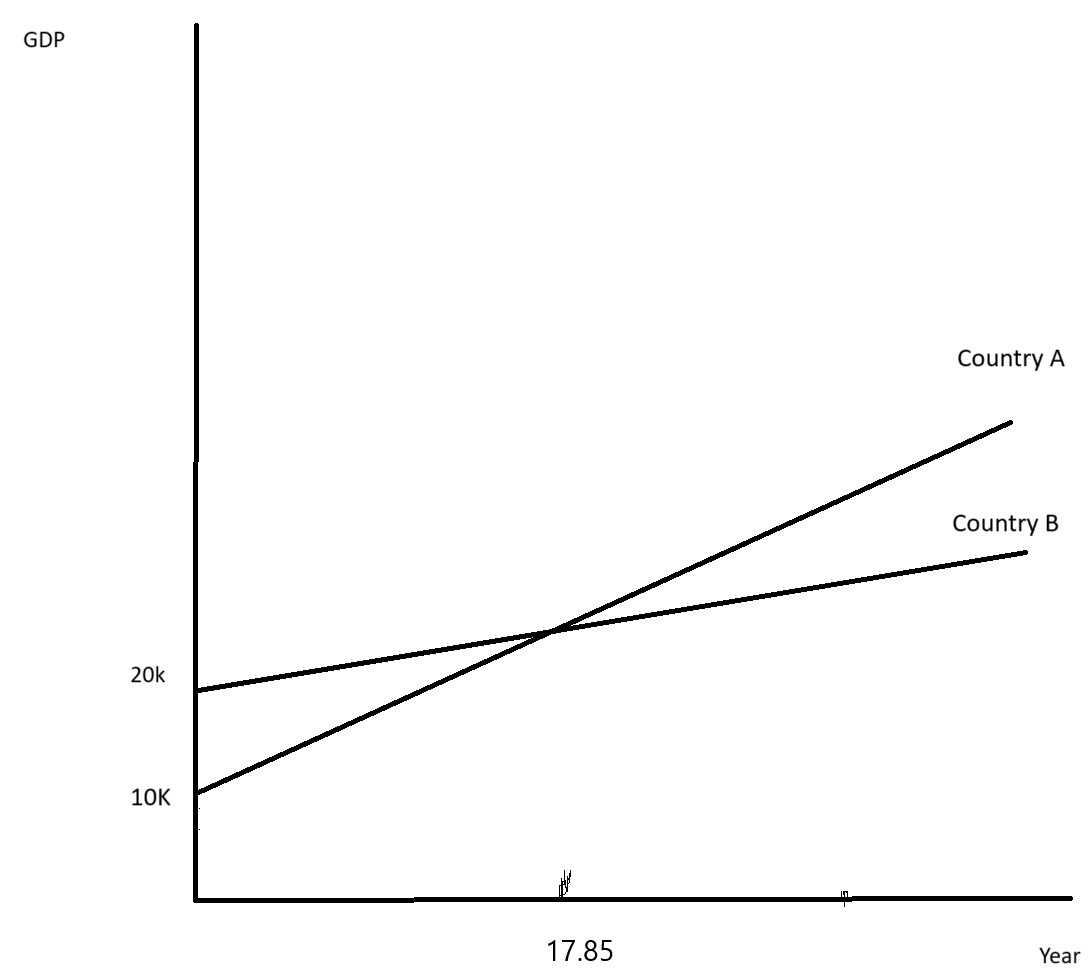
\includegraphics[width=0.7\linewidth]{figure/growth_two_countries}
	\end{figure}
	
\end{enumerate}

%\newpage
%%\begin{center}
%%	This page intentionally left blank. Please continue your answer for q.2 below.
%%\end{center}
%\vspace*{\fill}
%
\newpage

\item  \textbf{(10 pts)}\label{P3} Suppose \( x \), \( y \), and \( z \) grow at constant rates given by \( \bar{g}_x \), \( \bar{g}_y \), and \( \bar{g}_z \). What is the growth rate of \( z \) in terms of the growth rates of \( x \) and \( y \) in each of the following cases?
\begin{enumerate}[label=(\alph*)]
	\item (\textbf{3 pts}) $z=x^3 y$
	\item (\textbf{3 pts}) $z= \frac{y^{0.1}}{x^{0.5}}$
	\item (\textbf{4 pts}) $z=(4x)^{-0.2} \left(\frac{3}{y}\right)^{0.2}$
\end{enumerate}

\textbf{Solution}
\begin{enumerate}[label=(\alph*)]
	\item $g_z = 3g_x+g_y$
	\item $g_z = g(y^{0.1}x^{-0.5}) = 0.1g_y -0.5 g_x$
	\item $g_z = -0.2 g_x - 0.2 g_y$
	The $4$ and $3$ are constant numbers, so, the growth rate of those term are zero.
\end{enumerate}


\newpage

\item  \textbf{(15 pts)}\label{P4} Assume that the representative firm in a simple model economy is endowed with the production function $F(A,K,L) = A + K^\alpha L^\beta$ where $\alpha$ and $\beta$ are positive constants, $L$ is the labour employed, $K$ is the stock of capital, and $A$ is the stock of idea that effects productivity.

\begin{enumerate}[label=(\alph*)]
	\item  What restrictions are necessary for the values of $\alpha$ and $\beta$ for the production function to satisfy the ALL the following conditions? Show it mathematically.
	\begin{enumerate}[label=(\roman*)]
		\item Marginal product of labour is positive.
		%\item Marginal product of capital is positive
		\item Diminishing marginal product of labour
		%				\item Capital is necessary for production
		%				\item Labour is necessary for production
		%\item Constant returns to scale in labour and capital
	\end{enumerate}
	\clearpage
	\item Does this production function exhibit constant returns to scale if only labor and capital are allowed to vary? What if all three variables (A, L, K) are allowed to change? Show all steps in your explanation.
	
	\vspace{10cm}
	\item Based on the results in part (b), is this production function appropriate for the Romer growth model, where the function exhibits constant returns to scale in objects and increasing returns to scale in both objects and ideas? Explain why or why not in 2-4 sentences.
\end{enumerate}

\clearpage

\textbf{Solution:}
\begin{enumerate}[label=(\alph*)]
	\item 
	\begin{enumerate}[label=(\roman*)]
		\item For the marginal product of labor (MPL) to be positive, we require:
		\[
		\frac{\partial F(K,L)}{\partial L} = \beta  K^\alpha L^{\beta - 1} > 0
		\]
		Since  \(K\), and \(L\) are all positive:
		\[
		\beta > \frac{0}{ K^\alpha L^{\beta - 1}} = 0
		\]
		Therefore, for the MPL to be positive, we need \(\beta > 0\).
		
		
		\item For diminishing marginal product of labor, we need:
		\[
		\frac{\partial^2 F(K,L)}{\partial L^2} = \beta (\beta - 1)  K^\alpha L^{\beta - 2} < 0
		\]
		Since \(K\), and \(L\) are positive:
		\[
		\beta(\beta - 1) < 0
		\]
		This implies \(\beta - 1 < 0\), meaning \(\beta < 1\). Given \(\beta < 1\), the term \((\beta - 1)\) is negative. Dividing both sides of the inequality by \((\beta - 1)\), we find\footnote{The inequality flipped because of the negative term}:
		\[
		\beta > 0
		\]
		Thus, to have diminishing marginal product of labor, we require \(0 < \beta < 1\).
		
		
	\end{enumerate}
	\clearpage
	\item Let both \(K\) and \(L\) be multiplied by a factor \(a\):
	\[
	F(A, aK, aL) = A +  (aK)^\alpha (aL)^\beta = A+ a^{\alpha + \beta}  K^\alpha L^\beta
	\]
	Compare it to 
	\[aF(A, K, L) = aA + a K^\alpha L^\beta \]
	
	If $\alpha$ and $\beta$ is between zero to one and $\alpha+\beta = 1$,  this function is not a constant return to scale function.
	
	When $A$ is also allow to change and that $\alpha + \beta = 1$,
	\[
	F(aA, aK, aL) = aA +  (aK)^\alpha (aL)^\beta = aA+ a^{\alpha + \beta}  K^\alpha L^\beta = aF(A, K, L)
	\]
\end{enumerate}	

\clearpage
\item  \textbf{(15 pts)}\label{P5} 
According to our neoclassical production model, a country’s GDP per capita is determined by its total factor productivity (TFP) and the amount of capital per worker. The relationship is given by:

\[
y = \bar{A} k^{\frac{1}{3}}
\]

where \( y \) represents GDP per capita, \( k = \frac{K}{L} \) is capital per worker, and \( \bar{A} \) is total factor productivity (TFP).

Suppose we have data on GDP per capita, capital per worker, and an additional factor to be used later, comparing the country of Ikkousha to Ichiran. (use subscript $a$ to stand for Ikkousha and subscript $b$ to stand for Ichiran)

\begin{table}[htbp]
	\centering
	\begin{tabular}{l|ccc}
		Country & Observed y & Observed k & Observed m \\
		\midrule
		Ikkousha & 1.00  & 1.00  & 1.10 \\
		Ichiran & 0.40  & 0.95  & 0.30 \\
		\bottomrule
	\end{tabular}%
	\label{tab:addlabel}%
\end{table}%

\begin{enumerate}[label=(\alph*)]
	\item \textbf{(3 pts)} 
	Calculate the implied TFP in Ikkousha and Ichiran assuming our model fits the data exactly.
	\clearpage
	\item \textbf{(3 pts)} 	
	By looking at the difference in TFP and capital across the two countries. Which of these components accounts for the larger portion of the difference in economic performance? Explain in 2-4 sentence.
	
	\vspace{8cm}
	\item \textbf{(3 pts)} Does the results in part b) help us in developing economic policy to narrow the difference in economic performance? Why? Explain in 3-5 sentences.
	
	\clearpage
	\item \textbf{(3 pts)} Inspired by the work of Daron Acemoglu, a recent Nobel Laureate in Economics, a group of young researchers developed a new measure for institutional quality using data mining techniques, denoted as \( M \). If \( m = M/L \) represents the institutional quality per worker, our extended production function become:
	
	\[
	y = \bar{A} k^{1/3} m^{1/4}
	\]
	
	Calculate the implied TFP in Ikkousha and Ichiran, assuming our model perfectly fits the data.
	
	\vspace{5cm}
	\item \textbf{(3 pts)} By looking at the difference in TFP, capital and the quality of institution across the two countries in part d). Does the same component reported in part b) still account for the same portion of the difference in economic performance? Explain in 3-5 sentences.
\end{enumerate}

\clearpage

\clearpage
\textbf{Solution}
\begin{enumerate}[label=(\alph*)]
	\item 
	\[\bar{A} = \frac{y}{k^(1/3)}\]
	
	Using this formula, we have $A_a = 1$ and $A_b = 0.407$.
	
	\item 
	Comparing the capital across the two countries, we observe minimal differences of $\frac{k_A}{k_b} = 95\%$. However, the TFP in Ichiran is only 41\% of that in Ikkousha. Thus, we can conclude that TFP accounts for the majority of the difference in output.
	
	We can calculate the contribution of each factor more formally by 
	\[\frac{y_a}{y_b} = \frac{\bar{A_a}}{\bar{A_b}} \left(\frac{k_a}{k_b}\right)^{\frac{1}{3}}\]
	But, it is not required for this question. 
	
	\item It does not help in designing economic policies because TFP accounts for most of the difference in output, yet TFP is an indirect measure. After all, it is the residual term in the production function after we plug in the observable.  As a result, it is not possible to formulate policies directly based on TFP unless we make big assumption about what factor contribute to the difference in TFP. 
	
	\item Rearrange the formula:
	\[ \bar{A} = \frac{y}{k^{1/3} m^{1/4}}
	\]
	
	Now, the $A_a = 0.976$ and $A_b = 0.55$
	
	
	\item Now, the difference in TFP narrow to 56\% from 40\%. This indicates the TFP now contribute less than before in part b). Part of its previous explanation power went to the difference in quality of institution, which the difference is about 27\%. It is consistent with study that TFP would explain less as we add more variables to the production function.
\end{enumerate}

%\newpage
%\begin{center}
%	This page intentionally left blank. Please continue your answer below.
%\end{center}
%\vspace*{\fill}
%
%\newpage
%\begin{center}
%	This page intentionally left blank. Please continue your answer below.
%\end{center}
%\vspace*{\fill}

\newpage

\item  \textbf{(30 pts)}\label{P6}  This question relates to the Solow growth model discussed in Chapter 5. Liverpool, a closed economy with no government spending, operates under the following production function:
\[
Y_t = A K_t^{1/4} L_t^{3/4}
\]		
In this model, \(Y_t\) represents the output in period \(t\), \(K_t\) denotes the capital stock in period \(t\), and \(L_t\) stands for the labor employed in period \(t\). The accumulation of capital follows the standard equation:
\[
K_{t+1} = (1 - \delta) K_t + I_t
\]		
where \(\delta\) is the depreciation rate and \(I_t\) is the investment in period \(t\).

Liverpool's population saves a fixed proportion, \(\bar{s}\), of their output for investment each period. The population grows at a rate \(\bar{n}\), following the equation \(L_{t+1} = (1 + \bar{n}) L_t\). Lowercase letters represent per-person values of the variables.

\begin{enumerate}[label=(\alph*)]
	\item \textbf{(2 pts)} Convert the capital accumulation equation from aggregate to per-person terms. The left-hand side should equal \(\Delta k_{t+1}\), while the right-hand side should include \(y_t\), \(k_t\), and the relevant parameters.
	
	\clearpage
	\item \textbf{(3 pts)} Find the steady-state values of capital per capita (\(k^*\)) and output per capita (\(y^*\)).
	
	\vspace{12cm}
	\item \textbf{(3 pts)} What happens to output per capita in the steady state when \(\bar{s}\) increases? Use your findings from part (b) to explain.
	
	\clearpage
	\item \textbf{(4 pts)} Another economy, Claremont, has similar characteristics (i.e., identical parameters) but currently has a lower output than Liverpool. Meanwhile, Liverpool is in its steady state. How would we expect the growth rate of output in Claremont to compare with that of Liverpool? Why? Explain in 3-5 sentences and provide a rough real-world example.
	
	\vspace{5cm}
	\item \textbf{(3 pts)} Draw separate time graphs (on a ratio scale) for $Y$ and $y$, one for Liverpool and the other for Claremont (in total 4 graphs).
	
	\clearpage
	\item \textbf{(3 pts)} After learning the Solow model, the Liverpool government has contemplated encouraging increased savings among its citizens to stimulate economic growth. Will this approach be effective in the short run and in the long run? Provide a explanation in 3-5 sentences.
	
	\vspace{6cm}
	\item \textbf{(3 pts)} Draw a Solow diagram with \( k \) on the x-axis to illustrate the scenario described in part (f). Label all steady states, the initial level, and the movement of any variables.
	
	\clearpage
	\item \textbf{(2 pts)} Draw two separate time graphs (on a ratio scale) for $Y$ and $y$ to illustrate the scenario described in part (f).
	
	\vspace{10cm}
	\item \textbf{(4 pts)} Rather than encouraging higher savings, the Claremont government decided to make a one-time investment to increase Claremont’s capital stock in order to catch up with Liverpool, which now has a higher savings rate. Would this policy be effective in the short run and the long run? Explain in 3-5 sentences.
	
	\clearpage
	\item \textbf{(3 pts)} Draw a Solow diagram with \( k \) on the x-axis to illustrate the scenario of Claremont described in part (i). Label all steady states, the initial level, and the movement of any variables.
\end{enumerate}



\newpage
\textbf{Solution:}
\begin{enumerate}[label=(\alph*)]
	\item Plug in ($I_t = s Y_t$)
	\[K_{t+1}- K_t = \Delta K_{t+1}=  sY_t -\delta K_t\]
	Divide both side by $K_t$,
	\[\frac{\Delta K_{t+1}}{K_t} = g_K  = s\frac{Y_t }{K_t}-\delta = s\frac{Y_t/L_t }{K_t/L_t}-\delta = s\frac{y_t }{k_t}-\delta\]
	Now, recall that $k_t = \frac{K_t}{L_t}$ and apply the growth rate approximate formula:
	\[g_k = g_K - g_L\]
	
	Next, plug in the $g_K$ above and the fact that $g_L = \bar{n}$
	\[g_k= \frac{\Delta k_{t+1}}{k_t} = s\frac{y_t }{k_t}-\delta - \bar{n}\]
	Multiply both sides by $k_t$
	\[\Delta k_{t+1} = sy_t- (\delta + \bar{n})k_t\]
	\item 
	In steady state, $\Delta k_{t+1} = 0$
	\[0 = sy^*- (\delta + \bar{n})k^*\]
	\[(\delta + \bar{n})k^* = sy^* \]
	\[\frac{k^*}{y^*} = \frac{s}{\delta + \bar{n}} \]
	
	\clearpage
	Rearrange the equation to $k^* = \frac{s}{\delta + \bar{n}} y^*$ and plug it into the output function ($y_t = Ak^{1/4}_t$):
	\[y^* = A \left(\frac{s}{\delta + \bar{n}} y^*\right)^{1/4}\]
	\[y^{* 3/4} = A \left(\frac{s}{\delta + \bar{n}} \right)^{1/4}\]
	\[y^{*} = A^{4/3} \left(\frac{s}{\delta + \bar{n}} \right)^{1/3}\]

	
	The steady-state $k^*$ is then
	\[k^* =  A^{4/3}  \left(\frac{s}{\delta + \bar{n}} \right)^{4/3}\]
	
	\item Mathematically, when \(\bar{s}\) increases, the right-hand side of the equation rises, indicating that output per capita will increase in the steady state. An increase in \(s\) means the economy is investing more each period, which results in more capital being available in the future, ultimately leading to higher output.
	
	\item We would expect Claremont to have a higher growth rate. Since both economies share the same parameters, they will eventually converge to the same steady state. However, because Claremont currently has a lower output level, there will be positive net investment (i.e., \(sy_t > (\delta + \bar{n}) k_t\)), leading to capital growth in addition to population growth. According to the principle of transitional dynamics, an economy further below its steady state tends to grow faster.
	
	We observe that, among OECD countries, economy with a lower GDP would grow faster while the country with higher GDP would grow slower.
	
	\item Claremont would have a higher growth rate initially. Meanwhile, Liverpool is always on its steady state for output per capita, and a constant growth at $\bar{n}$ for total output.
	\begin{figure}[htbp!]
		\centering
		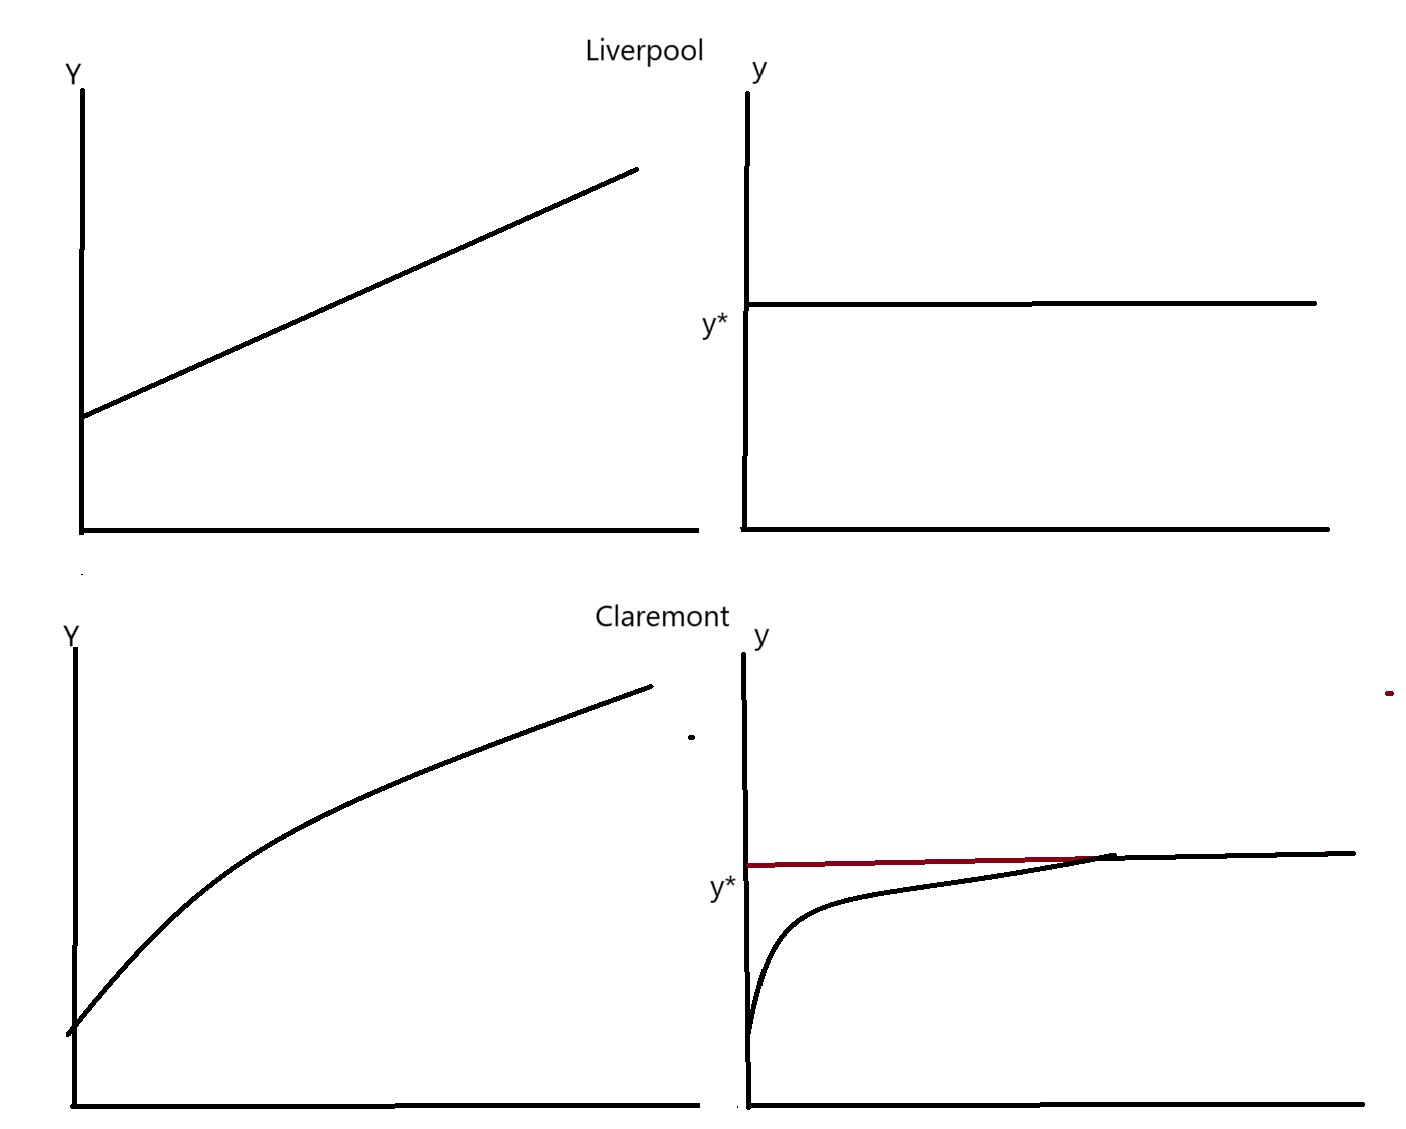
\includegraphics[width=0.7\linewidth]{figure/screenshot001}
	\end{figure}
	
	\clearpage
	\item In the short run, an increase in savings can lead to higher investment, which, in turn, can lead to a greater capital accumulation. As well, the higher saving rate would increase the steady state value for all K, Y and y. Together, the economy can achieve a short run boost in growth. However, in the long run, diminishing returns to capital implies less and less to output growth as the capital accumulation. It will eventually converge to the point there are no additional capital would be accumulated. That is, we have converge to the steady state, where all variable does not change any more. Therefore, increased savings can stimulate in the short run, but it does not effect on the growth in the long run.
	
	\item An increase in $\bar{s}$ would cause the investment curve to shift up.
	\begin{figure}[htbp!]
		\centering
		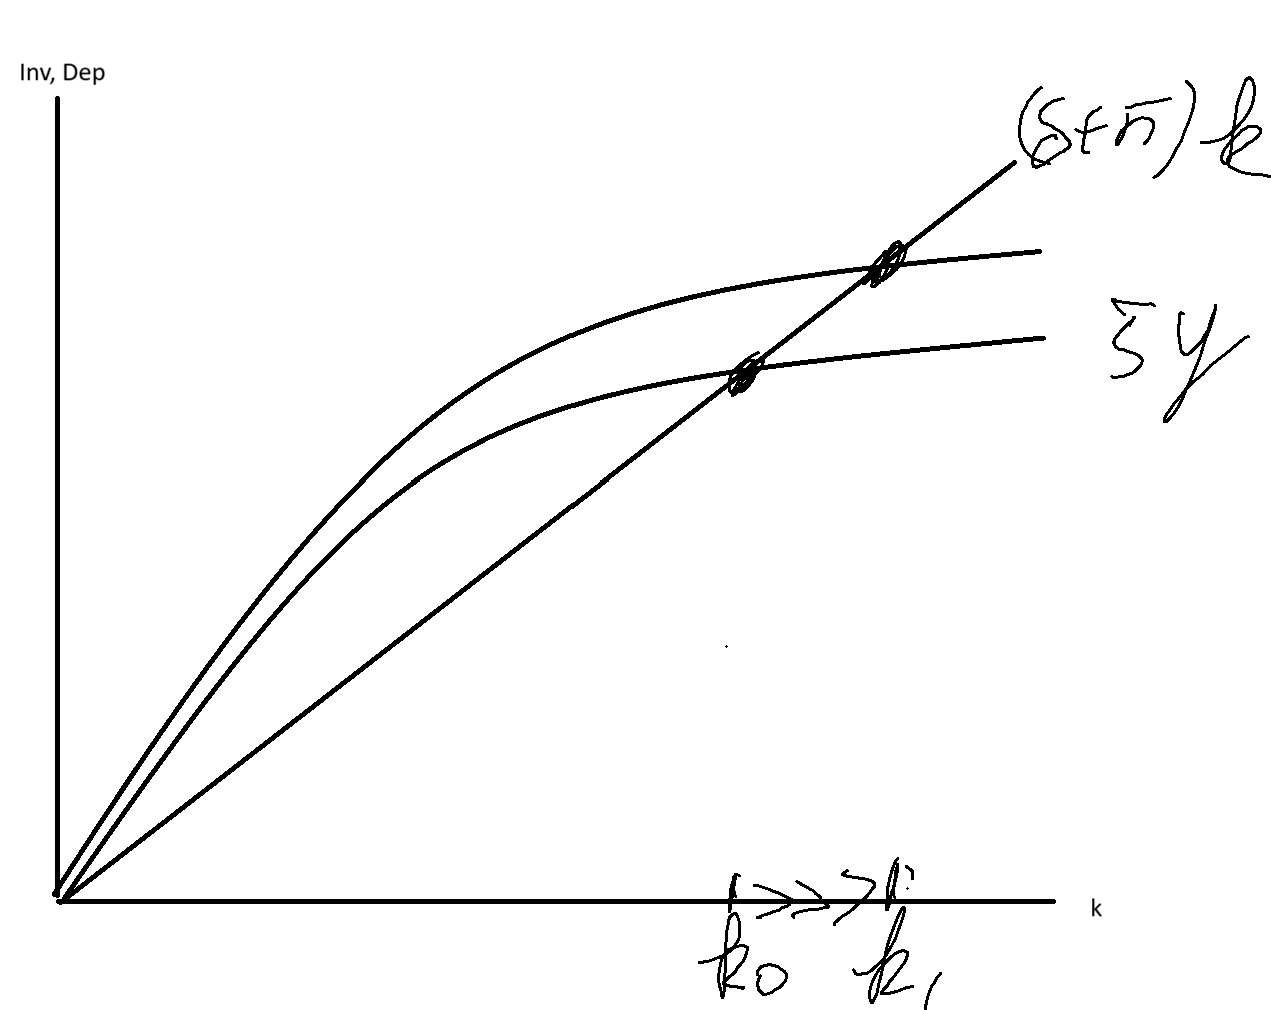
\includegraphics[width=0.7\linewidth]{figure/screenshot002}
	\end{figure}
	
	\clearpage
	\item The Y would grow at rate of $\bar{n}$ in steady state. It would grow faster after an increase in $\bar{s}$.
	
	\begin{figure}[htbp!]
		\centering
		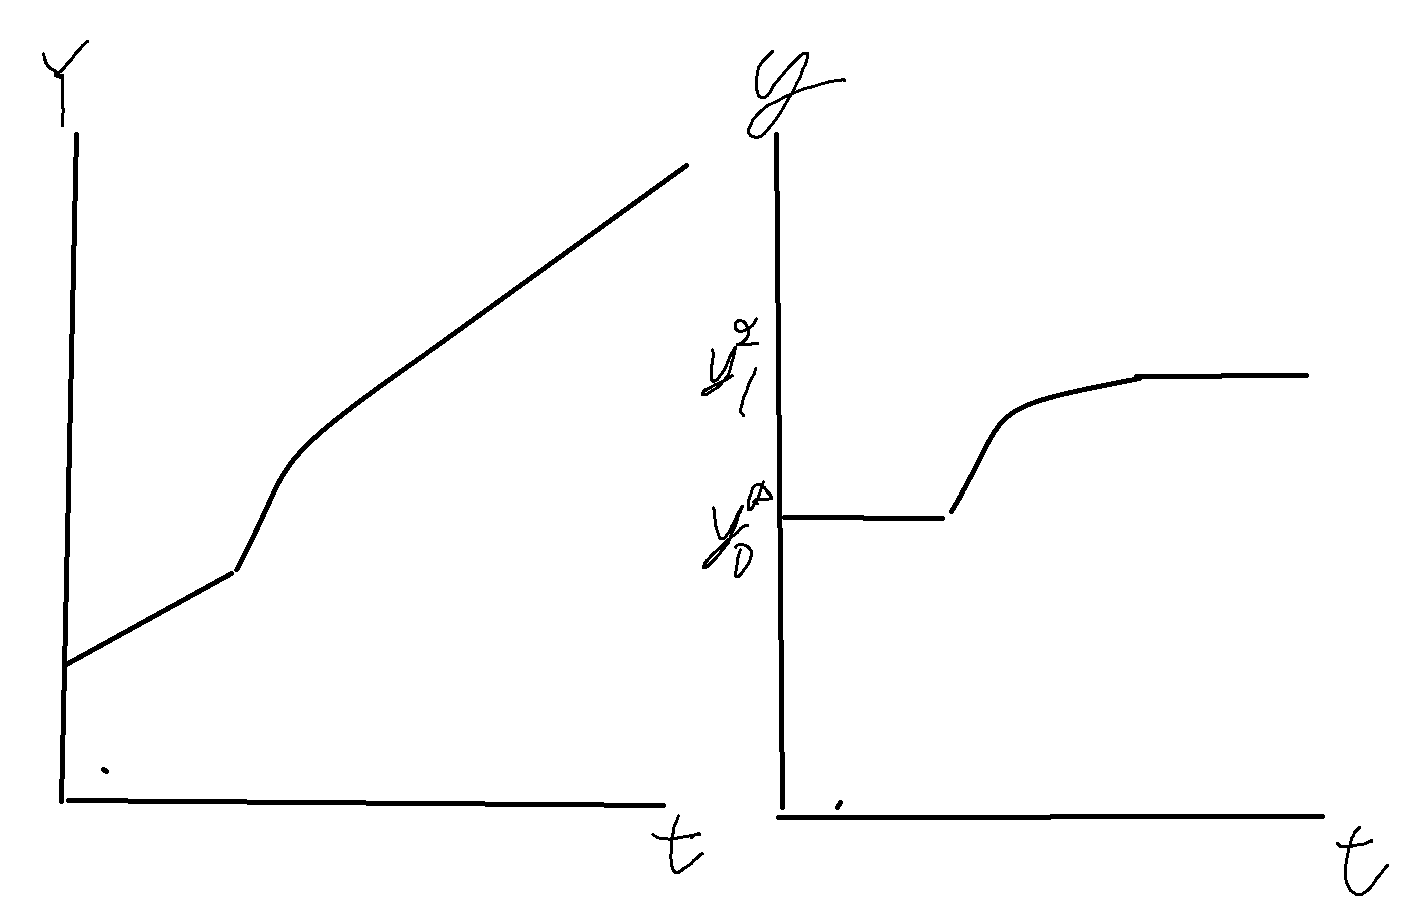
\includegraphics[width=0.7\linewidth]{figure/screenshot004}
	\end{figure}
	
	\clearpage
	\item When Claremont increases its capital stock through a one-time investment, it results in a higher level of output (and output per capita). However, according to the model, Claremont's capital per worker ($k$) above its steady state. By the principle of transitional dynamics, $k$ would decrease rapidly at first and then the decline would get slower as it approaches the steady state. Consequently, this policy is not effective in either the short or long term. In the short term, it raises the level of output but does not affect the growth rate of output. In the long term, this policy does not alter the steady-state value, meaning that output eventually returns to its original steady-state level.
	
	
	\item Initially, the $k$ would move above the steady state. Then, converge back to the steady state.
	\begin{figure}[htbp!]
		\centering
		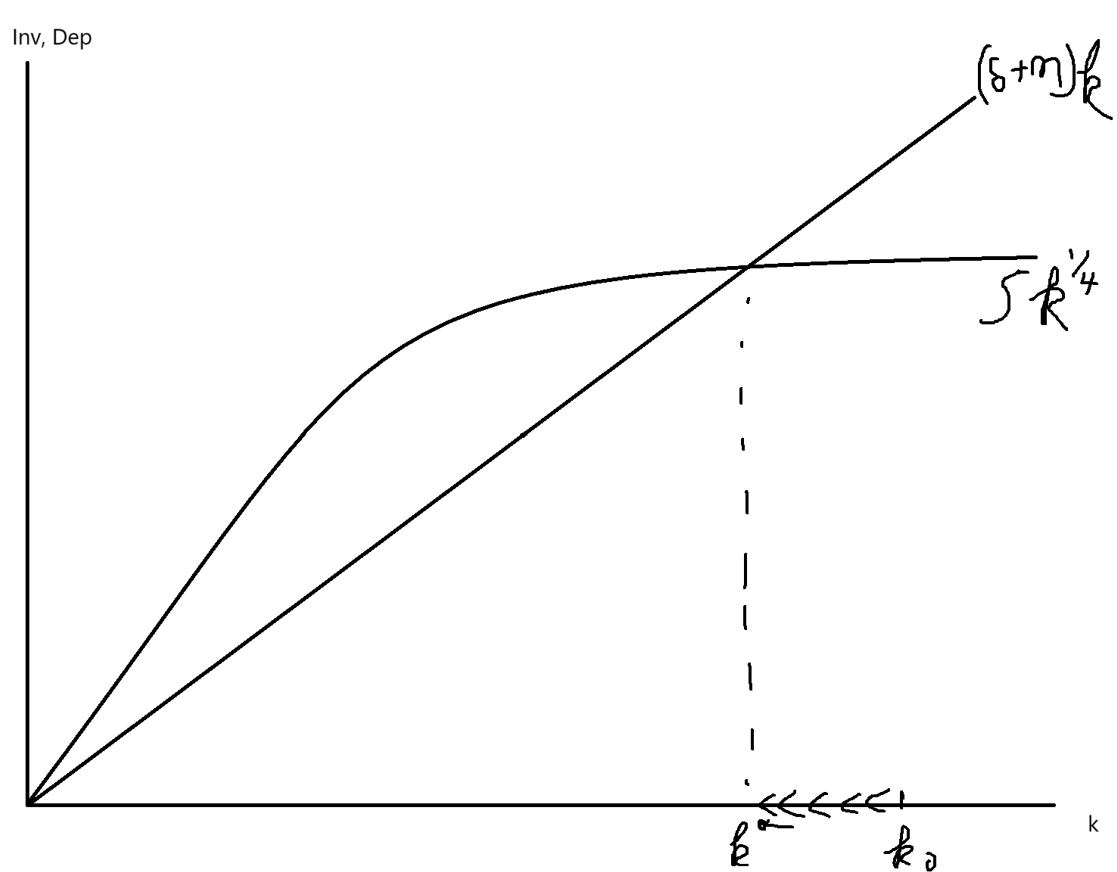
\includegraphics[width=0.7\linewidth]{figure/screenshot005}
	\end{figure}
	
\end{enumerate}
	
	
	
	

\newpage
\begin{center}
	This page intentionally left blank. Please continue your answer below.
\end{center}
\vspace*{\fill}
%
%\newpage
%\begin{center}
%	This page intentionally left blank. Please continue your answer below.
%\end{center}
\vspace*{\fill}

\centering{-- The End -- }
\end{enumerate}
  \end{document}
